\graphicspath{{img/appendix}{img/impl}}

\newcommand\invisiblesection[1]{%
  \refstepcounter{chapter}%
  \addcontentsline{toc}{chapter}{\protect\numberline{\thechapter}#1}%
  \sectionmark{#1}}

\invisiblesection{Hyperparameter Optimization}
\clearpage
\subsubsection{Hyperparameter Optimization Plots (moving avg. of 8)}
\label{app:hyperparam_optim}
\begin{figure}[H]
    \advance\leftskip-2.3cm
    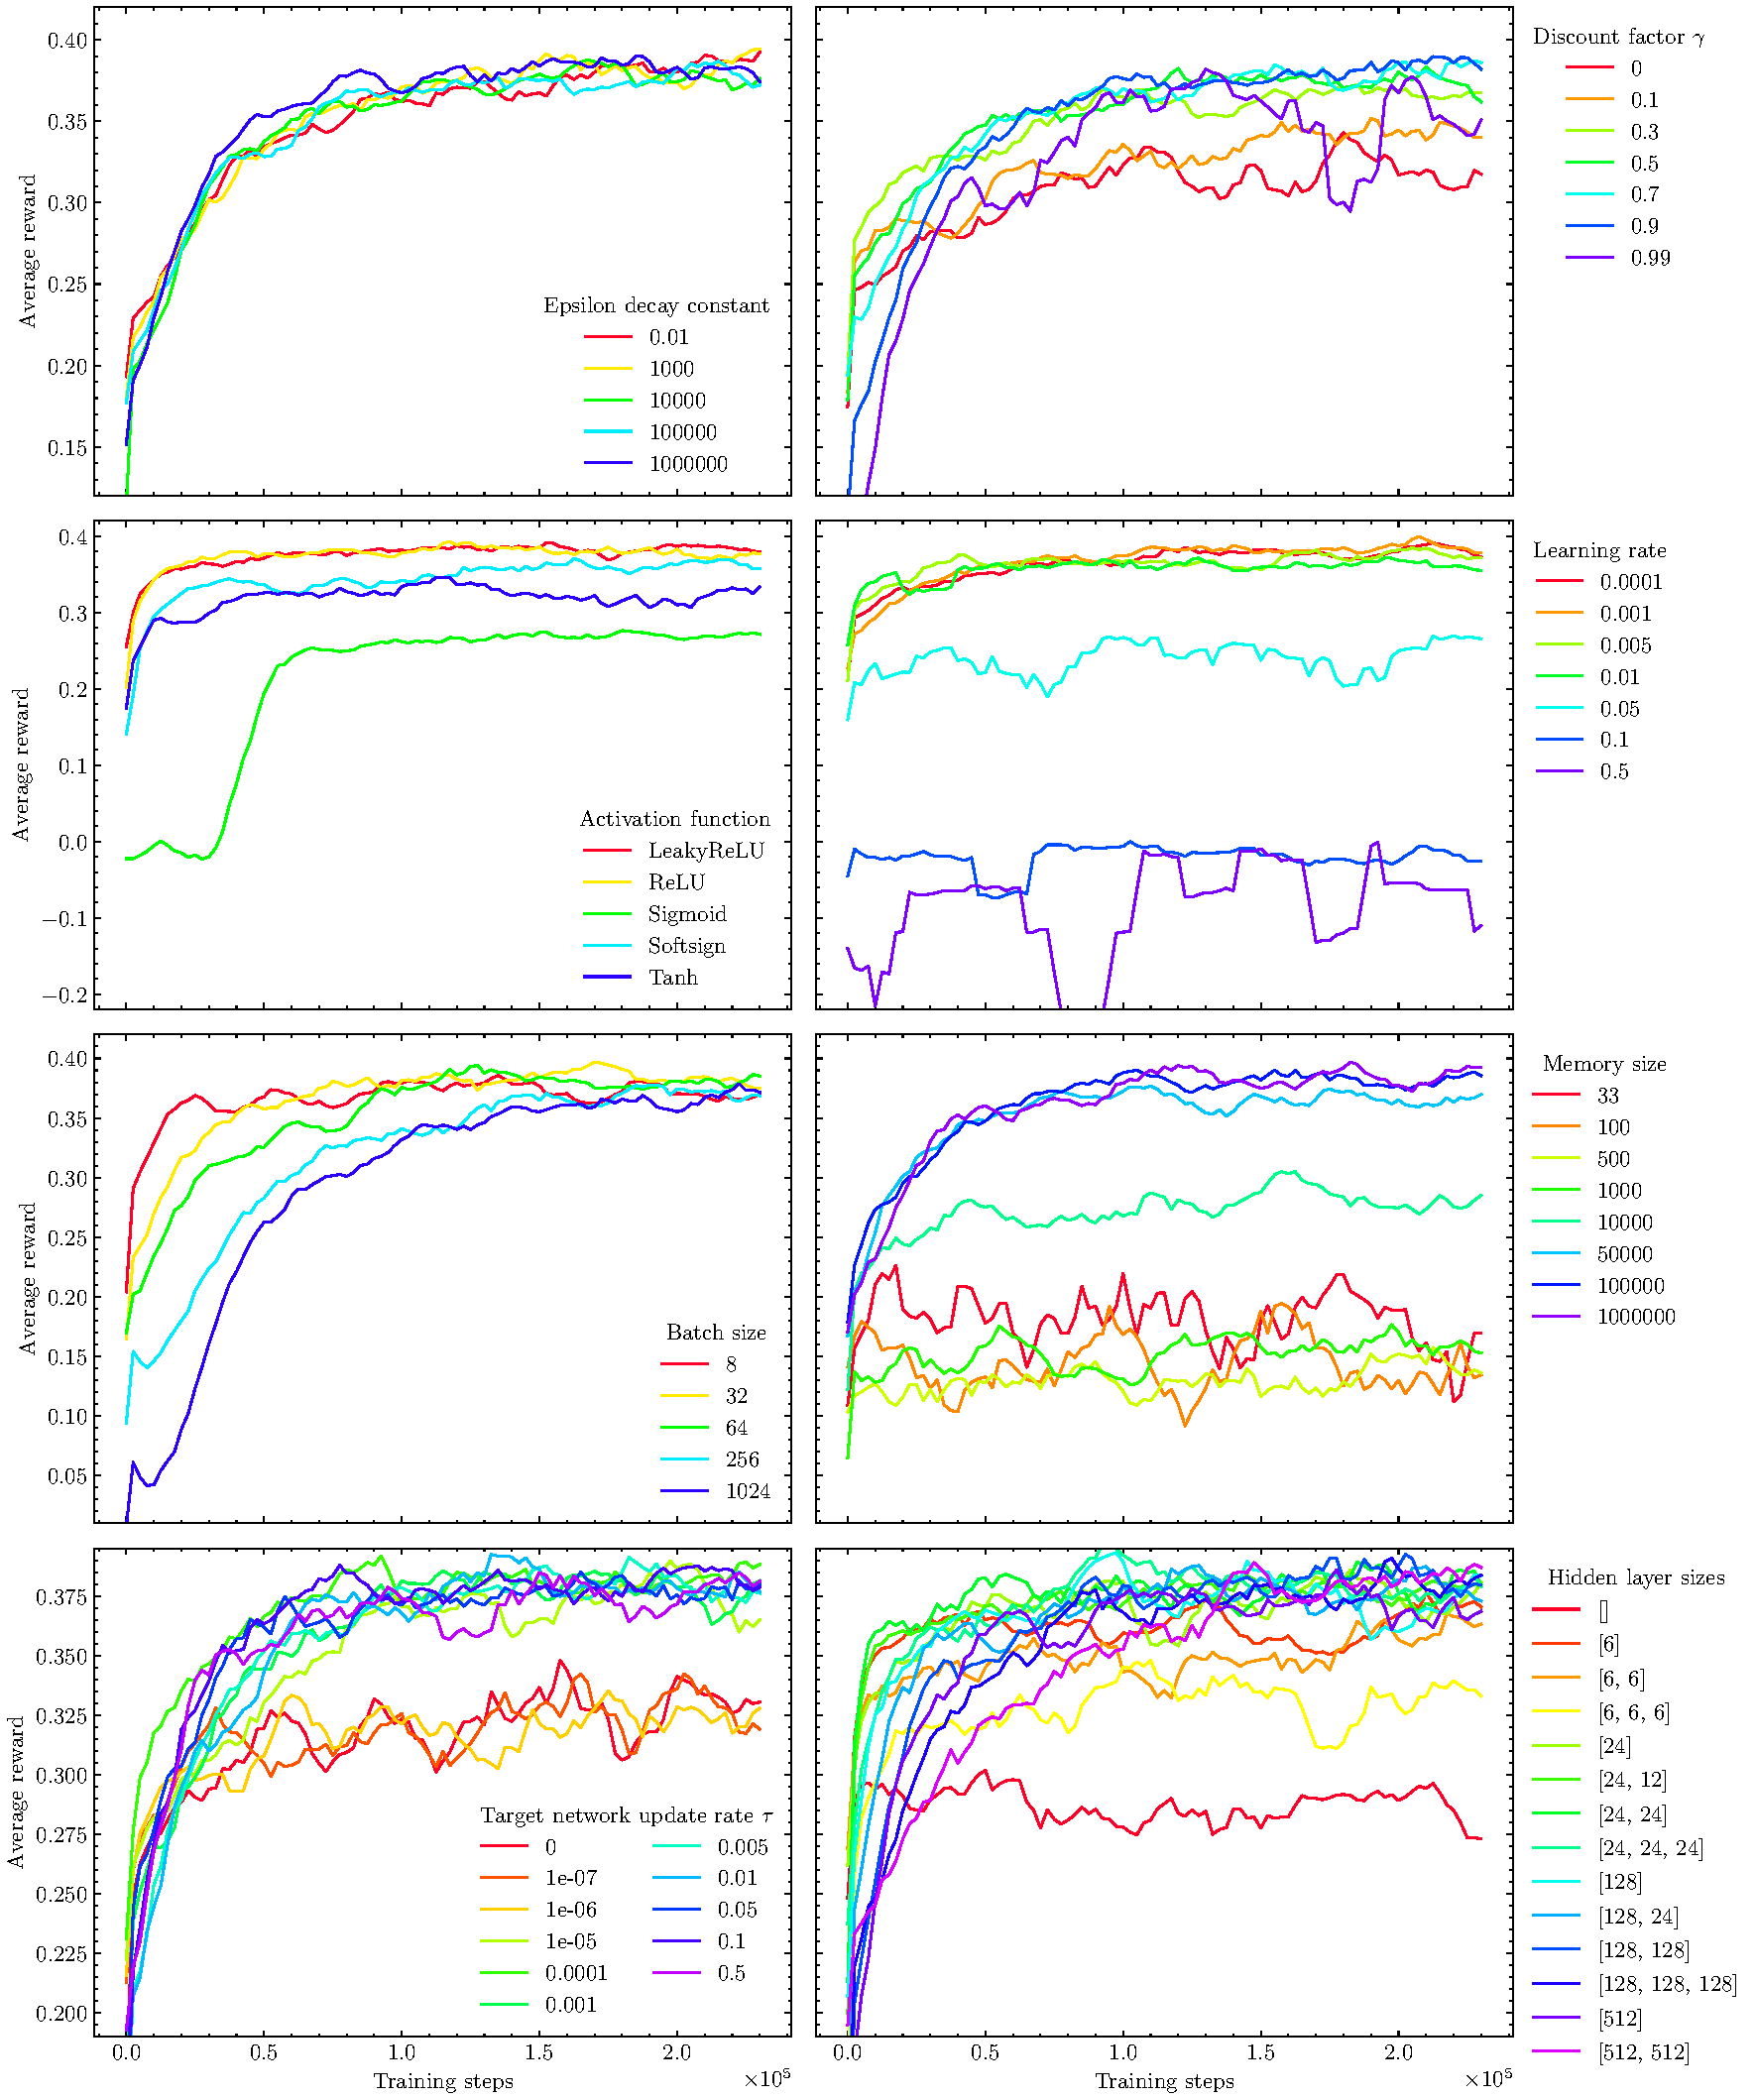
\includegraphics[width=1.28\textwidth]{hyperparam_optim_8_sci.pdf}
    \caption{Hyperparameter optimization plots analyzed in section \ref{sec:hyperparam_optim}.}
    \label{fig:hyperparam_optim_8}
\end{figure}

\subsubsection{Hyperparameter Optimization Plots (moving avg. of 30)}
\label{app:hyperparam_optim_30}
\begin{figure}[H]
    \advance\leftskip-2.3cm
    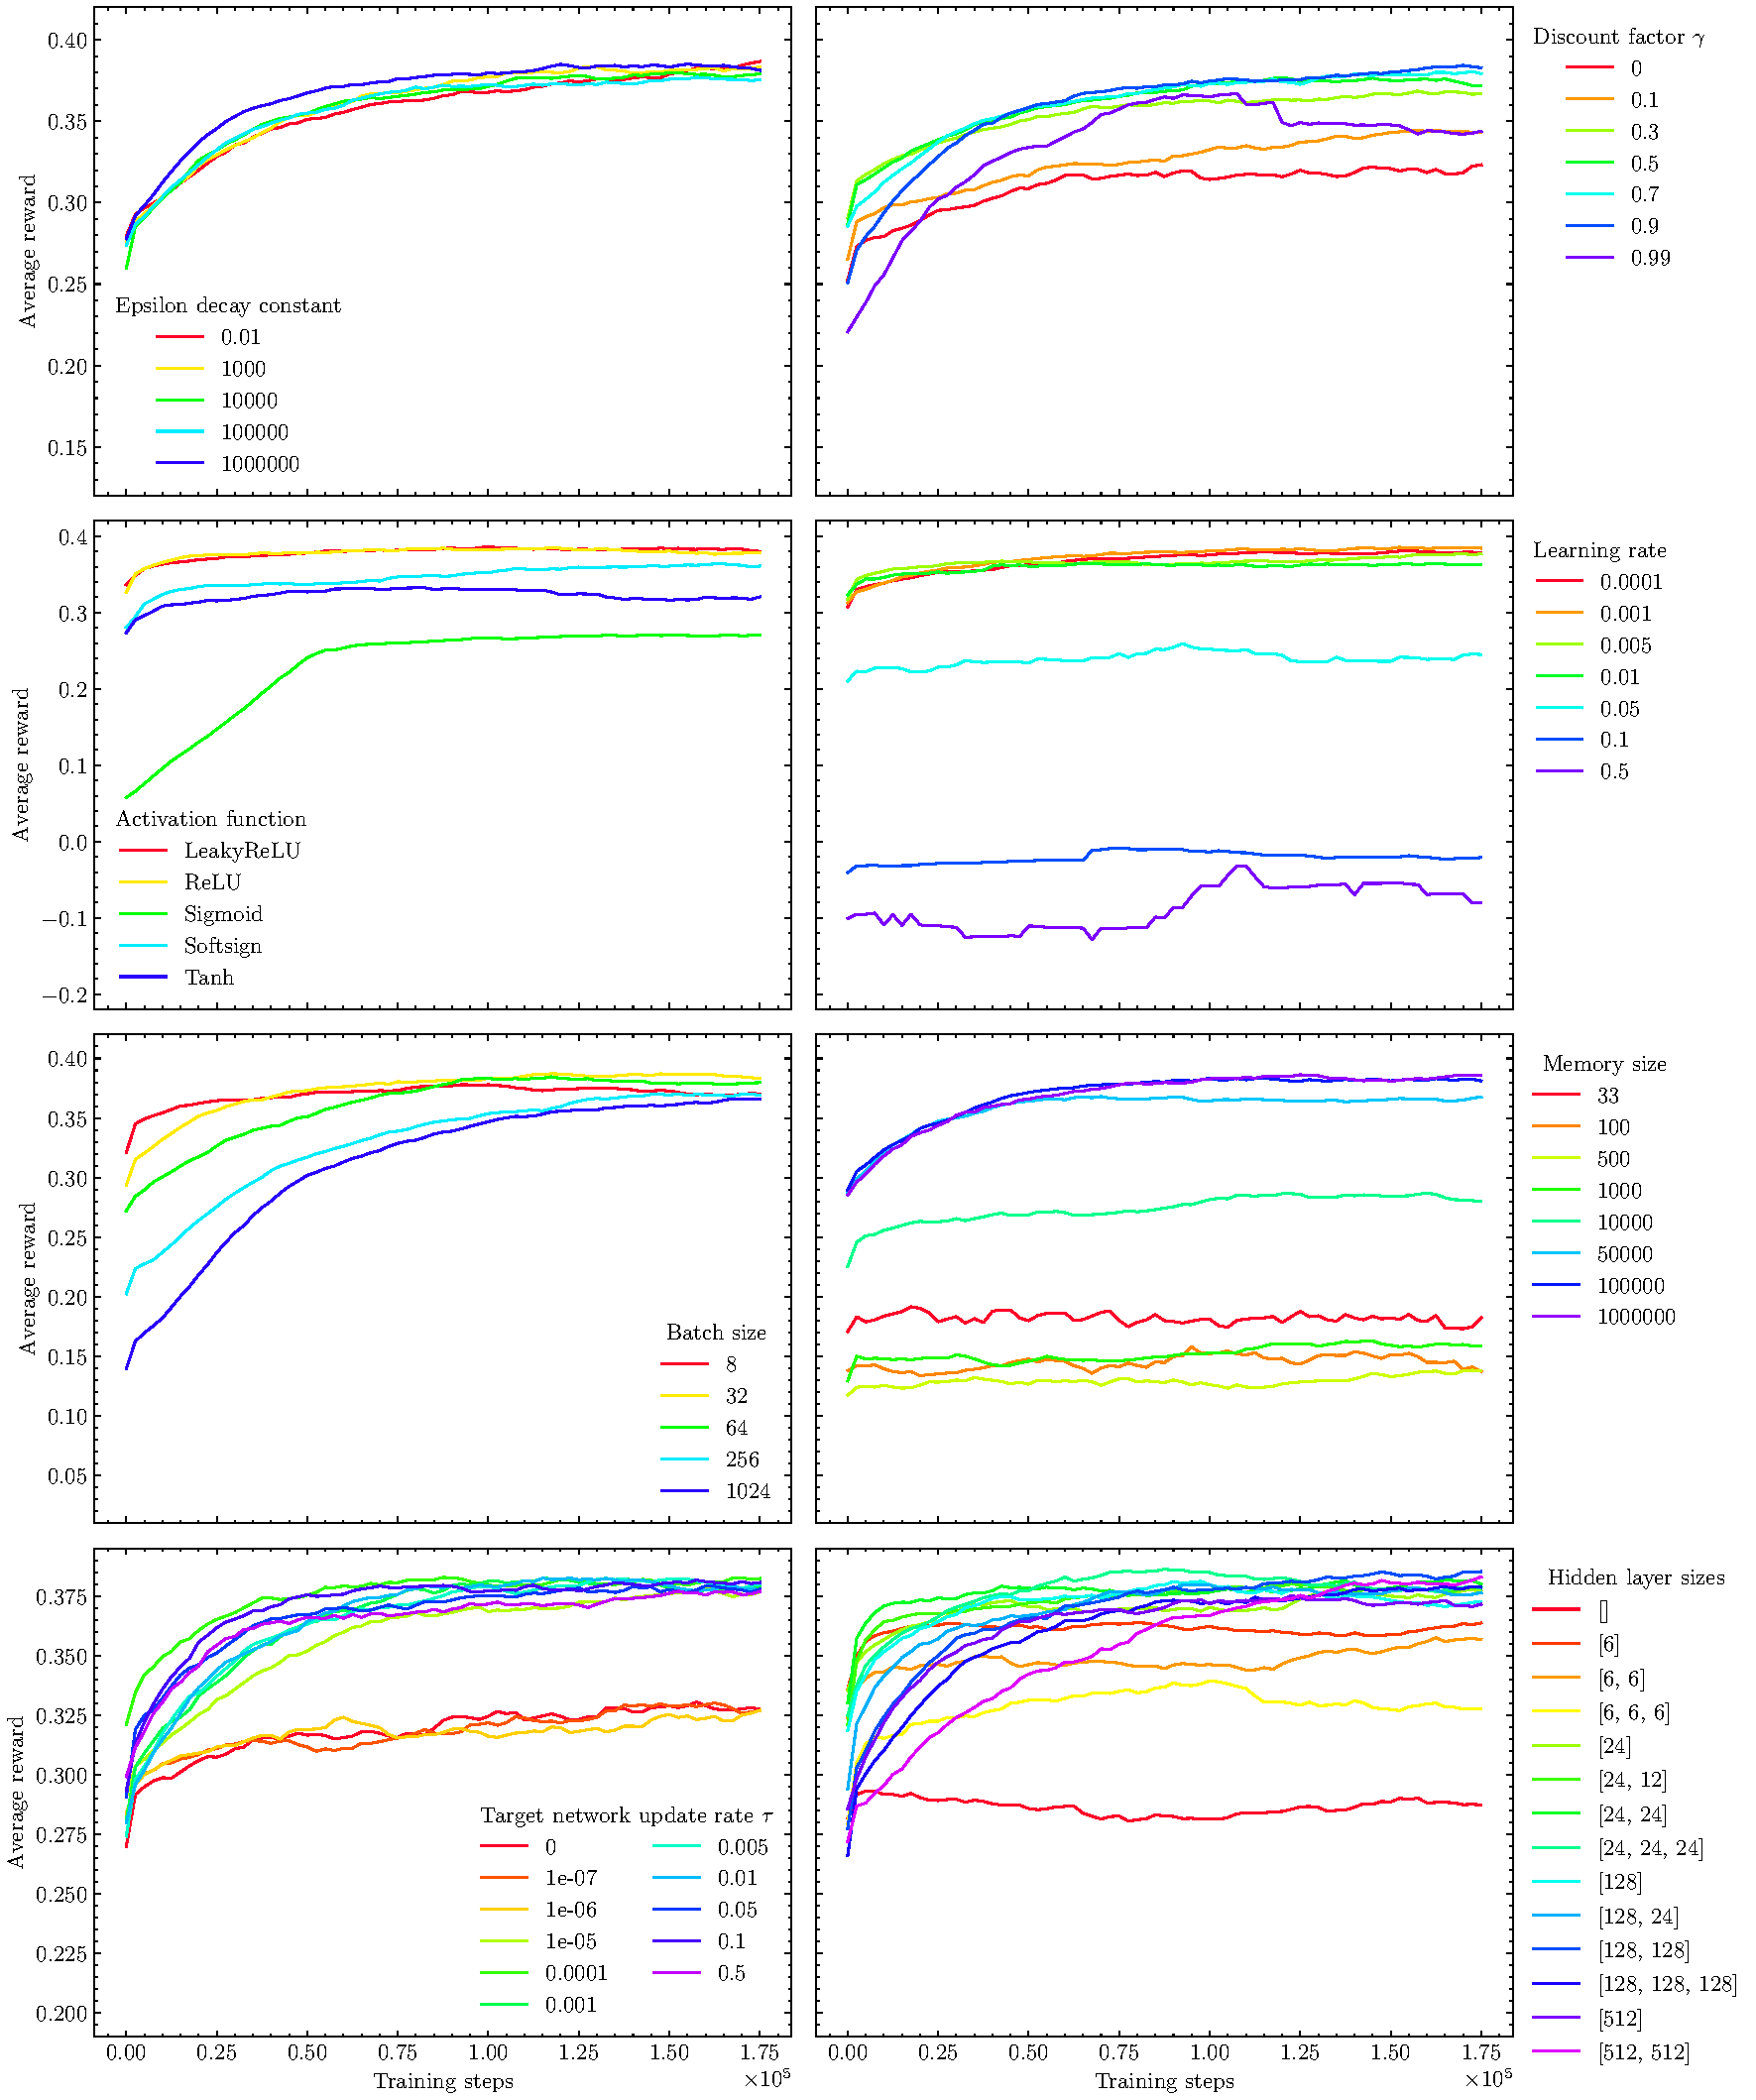
\includegraphics[width=1.28\textwidth]{hyperparam_optim_30_sci.pdf}
    \caption{Hyperparameter optimization plots analyzed in section \ref{sec:hyperparam_optim}.}
    \label{fig:hyperparam_optim_30}
\end{figure}


\chapter{Code}
\label{app:code}
only for reproducibility
rest of code is on github, packasge easy to use
setup like this
\section{First training}
\label{app:first_training}
\begin{minted}{python}
  from Trainer import Trainer, Hyperparams, EnvParams

  if __name__ == '__main__':
      envParams = EnvParams(render_mode="human",
                            length=128,
                            width=24,
                            moves_per_timestep=200,
                            window_height=200,
                            observation_distance=3,
                            distinguishable_particles=True,
                            initial_state_template="checkerboard",
                            social_reward=True,
                            # density=0.5,
                            use_speeds=True,
                            sigma=0.0001,
                            allow_wait=True,
                            invert_speed_observation=True,
                            speed_observation_threshold=0.35,
                            #punish_inhomogeneities=True,
                            #inh_rew_idx=1,
                            #speed_gradient_reward=False,
                            #binary_speeds=True,
                            #choices=4,
                            # speed_gradient_linearity=0.1,
                            )
      hyperparams = Hyperparams(BATCH_SIZE=32,
                                GAMMA=0.85,
                                EPS_START=0.9,
                                EPS_END=0.05,
                                EPS_DECAY=100_000,
                                TAU=0.005,
                                LR=0.001,
                                MEMORY_SIZE=500_000)
  
      trainer = Trainer(envParams, hyperparams, reset_interval=100_000,
                        total_steps=500_000, do_plot=True, plot_interval=4000, new_model=True)
  
      trainer.train_and_save()
\end{minted}

\section{Second training}
\label{app:second_training}
\begin{minted}{python}
# import sys
# sys.path.append('src/SmartTasep/') # uncomment this line if PYTHNONPATH is not set in IDE
from Trainer import Trainer, Hyperparams, EnvParams

if __name__ == '__main__':
    envParams = EnvParams(render_mode="human",
                          length=128,
                          width=24,
                          moves_per_timestep=200,
                          window_height=200,
                          observation_distance=3,
                          distinguishable_particles=True,
                          initial_state_template="checkerboard",
                          social_reward=True,
                          # density=0.5,
                          use_speeds=True,
                          sigma=10,
                          allow_wait=True,
                          invert_speed_observation=True,
                          speed_observation_threshold=0.35,
                          #punish_inhomogeneities=True,
                          #inh_rew_idx=1,
                          #speed_gradient_reward=False,
                          #binary_speeds=True,
                          #choices=4,
                          # speed_gradient_linearity=0.1,
                          )
    hyperparams = Hyperparams(BATCH_SIZE=32,
                              GAMMA=0.85,
                              EPS_START=0.9,
                              EPS_END=0.05,
                              EPS_DECAY=100_000,
                              TAU=0.005,
                              LR=0.001,
                              MEMORY_SIZE=500_000)

    trainer = Trainer(envParams, hyperparams, reset_interval=100_000,
                      total_steps=500_000, do_plot=True, plot_interval=4000, new_model=True)

    trainer.train_and_save()
\end{minted}

